\documentclass[11pt]{article}

\usepackage{extras} % Se extras.sty

\begin{document}

\begin{center}

{\Huge\bfseries Testprotokoll}
\vspace{4em}
\end{center}

\begin{flushleft}


\begin{figure}[htbp]
\centering
\noindent\resizebox{.4\linewidth}{!}{
	\documentclass[border=10px]{standalone}
\usepackage{tikz}
\usetikzlibrary{patterns}
\usetikzlibrary{shapes.arrows}
\usepackage{amssymb}
\begin{document}
	
\begin{tikzpicture}[scale=1]
		
		\draw[thick] 	(0,0) -- (0,1);
		\draw[thick] 	(0,0) -- (2,0);
		\draw[thick] 	(3,2) -- (3,3);
					
		\draw[thick,pattern=north west lines, pattern color=black]	 	(0,1) -- (1,1) -- (1,4) -- (0,4) -- (0,1);
		
		%\draw[thick,pattern=north west lines, pattern color=black]
		%				(0,3) -- (3,3) -- (3,4) -- (1,4)
		%			--	(1,7) -- (0,7) -- (0,3);
		
		%\draw[thick,pattern=north west lines, pattern color=black]
		%				(2,5) -- (3,5) -- (3,6) -- (2,6)
		%			--	(2,5);
					
		\draw[thick,pattern=north west lines, pattern color=black]		(3,3) -- (2,3) -- (2,4) -- (3,4)
					--	(3,3);
					
		\draw[thick,pattern=north west lines, pattern color=black]
				(3,0) -- (2,0) -- (2,2) -- (3,2) -- (3,0);
				
		\draw[thick,->] (1.5,4) -- (1.5,3.5);
		
		%\draw[thick] (4.2,2.2) rectangle (5,2.8) node[pos=.5] {\tiny Robot};
		%\draw[thick] (1.2,6.2) rectangle (1.8,6.8);
		%\draw[thick,<-] (1.8,6.5) -- (2.3,6.5) node[right] {\tiny Nödställd};
		%\draw[thick, <-,overlay] (5.1,2.5) [out=0,in=-45] to (7,4) node [right=.5em] {\tiny Bluetooth\textsuperscript{\circledR}};
		\draw[thick,->,overlay] (7,4) [out=125,in=180] to (9,5) ;
		%\node[]  at (10,5) {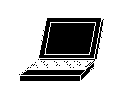
\includegraphics[scale=0.8]{laptop}};
		\node[overlay] at (10,4) {Datormodul};
	\end{tikzpicture}
	
\end{document}}
	\caption{Översikt av testbana\label{bana}}	
\end{figure}

\begin{description}
\item[Vad som har testats] \hfill \\
Test av reflexsensor för att se hur väl denna kan uppskatta en moduls längd (40 cm). Testade även rotation och stoppsträcka på underlaget i gamla TekNat-biblioteket. Därtill så testades också kartritningen på datormodulen. 
\vspace{1em}
\item[Utfall] \hfill \\
Uppskattningen av modullängd var bra! Underlaget i TekNat-biblioteket är dock ett problem, friktionen mellan hjul och underlag är inte tillräcklig vilket gör att roboten glider vid rotation. Kartritningen ritade dessutom ut för många moduler i djup på korridoren. 
\vspace{1em}
\item[Eventuella komplikationer] \hfill \\
Det faktum att roboten roterar för mycket vid rotation är ett problem (beroende på den dåliga friktionen mellan hjul och golv). Komplikationen med kartritningen kunde emellertid lösas på plats.
\vspace{1em}
\item[Hur arbetet fortskrider] \hfill \\
Testkörningar av roboten i banmiljö kommer att fortsätta under veckan. Olle undersöker möjligheten att eventuellt trä gummisnoddar på hjulen för öka friktionen vid rotation. Bör vara undersökt innan slutet av denna vecka.
\end{description}

\end{flushleft}

\end{document}